\chapter{Resultados}
\label{chap:resultados}

Este capítulo presenta las medidas del banco y las contrasta con el modelo del
capítulo~\ref{chap:modelo}. El resultado central es que, sobre el recorrido que el mecanismo hace
realmente con carga, \textbf{el par del tambor es prácticamente plano}, y que el perfil que lo
explica no es la espiral tal y como está descrita en la configuración, sino esa misma espiral
precedida por su arco de radio constante.

\section{Campañas de ensayos}
\label{sec:res-campania}

Los datos que sostienen el capítulo son los diez ensayos del 14 de octubre de 2026, todos con la
misma configuración y el mismo ciclo B$\to$A$\to$B. No se ha descartado ninguno: los diez recorren
\SI{1.80}{rev} de motor con una desviación típica de \SI{0.011}{rev} ---un \SI{0.6}{\percent}--- y
sus curvas se superponen dentro del espesor de la línea.

\begin{table}[H]
\centering
\caption{Ensayos del 14 de octubre de 2026. Los diez son consecutivos, tomados en menos de tres
minutos y con la misma configuración.}
\label{tab:ensayos}
\small
\begin{tabular}{@{}lcc@{}}
\toprule
Ensayo & Muestras & Recorrido (rev de motor) \\
\midrule
18:56:10 & 272 & 1,81 \\
18:56:24 & 276 & 1,79 \\
18:56:40 & 276 & 1,80 \\
18:56:55 & 276 & 1,78 \\
18:57:09 & 272 & 1,79 \\
18:57:24 & 272 & 1,78 \\
18:57:38 & 272 & 1,78 \\
18:57:53 & 272 & 1,80 \\
18:58:09 & 272 & 1,80 \\
18:58:48 & 272 & 1,80 \\
\bottomrule
\end{tabular}
\end{table}

Las campañas anteriores (septiembre y 7 de octubre) se interpretaron, las primeras, con el modelo de
punto de salida fijo, hoy superado. La del 7 de octubre, ya con el modelo tangente, da los mismos
resultados que la que aquí se presenta ---la meseta ajustada coincide en \SI{61}{\degree} y el orden
de las hipótesis es idéntico---, con peor repetibilidad. Sus conclusiones
geométricas no se mantienen y no se reproducen aquí; lo que sí se mantiene de ellas es la
caracterización de la cadena de adquisición, que no depende del modelo.

\section{Temporización del lazo de control}
\label{sec:res-temporizacion}

El firmware trabaja con un periodo fijo de \SI{50}{\milli\second}. Sobre las muestras de los ocho
ensayos, el periodo medido es de \SI{50.02}{\milli\second} con una desviación típica de
\SI{0.13}{\milli\second}, y el \SI{98.3}{\percent} de los intervalos caen dentro de
\SI{\pm 0.5}{\milli\second}. El tiempo de trabajo declarado por el propio lazo es de
\SI{10.96}{\milli\second} de media y \SI{11.00}{\milli\second} como máximo: un
\SI{22}{\percent} del periodo, con \SI{39}{\milli\second} de holgura.

Esa holgura importa porque la base de tiempos es lo que permite emparejar posición, fuerza y par en
la misma muestra. Un lazo que se saltara periodos desplazaría unas magnitudes respecto de otras y
contaminaría justo la comparación que se quiere hacer.

\section{Ensayo tipo}

La figura~\ref{fig:ensayo-tipo} muestra el último ensayo de la campaña. La secuencia es siempre la
misma: el eje arranca en B y avanza hacia A; durante la primera media vuelta larga el cable aún no
tira y las tres señales están en reposo; a partir de ahí la carga entra, la célula sube y el par se
estabiliza; al llegar al final de carrera el ciclo invierte y vuelve a B recorriendo los mismos
puntos en sentido contrario.

\begin{figure}[tbp]
\centering
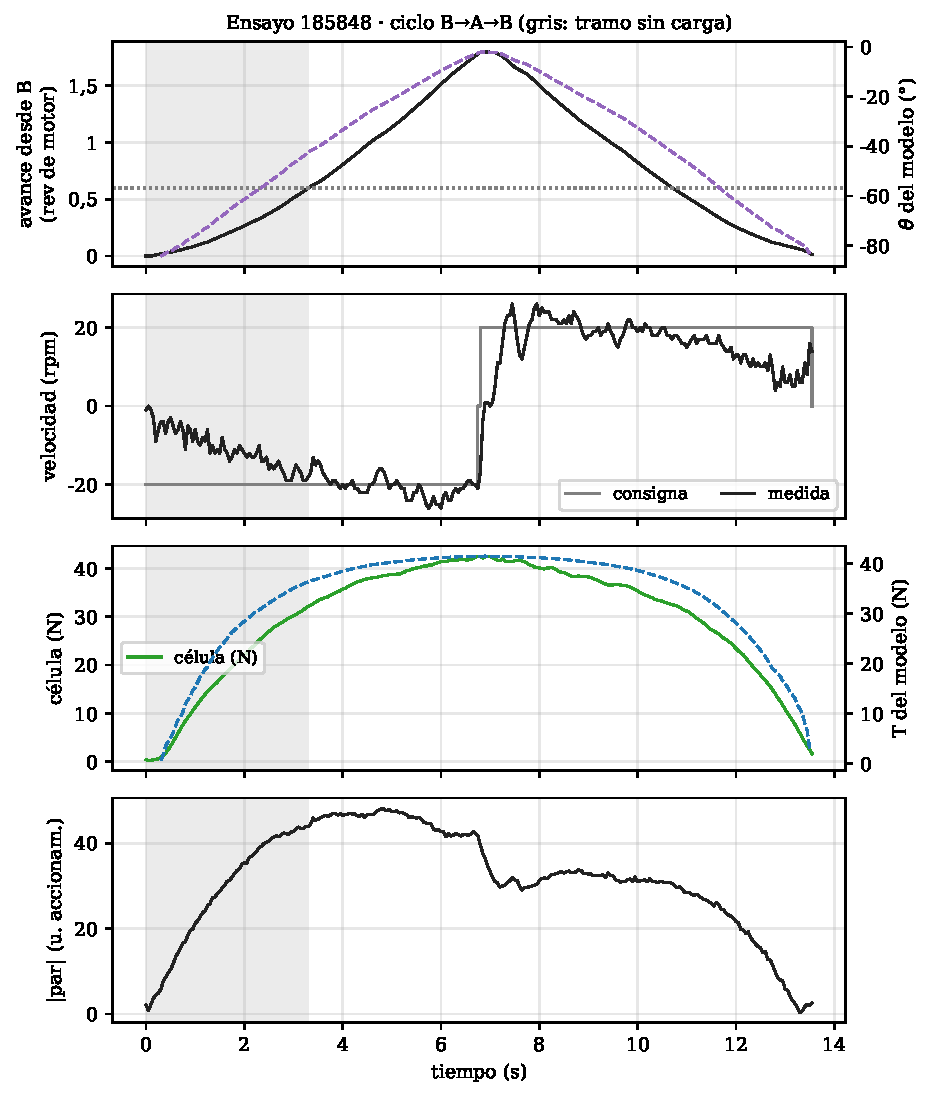
\includegraphics[width=\textwidth]{n14_ensayo_tipo.pdf}
\caption{Ensayo del 14 de octubre a las 18:58:48. De arriba abajo: avance del motor con el ángulo de
la barra que predice el modelo, velocidad frente a consigna, célula de carga frente a la tensión del
modelo, y par del accionamiento. La banda gris es el tramo en que el cable todavía no tira.}
\label{fig:ensayo-tipo}
\end{figure}

El tramo sin carga no es un defecto del ensayo sino una propiedad del mecanismo: en B la barra está a
\SI{-87}{\degree}, apenas \SI{2.6}{\degree} por debajo del reposo libre
$\theta_{\text{libre}} = \SI{-84.4}{\degree}$ de la ecuación~\eqref{eq:libre}, y ahí el brazo de la
pesa es casi nulo. El mecanismo, sencillamente, no necesita fuerza para sostenerla. Todo el análisis
cuantitativo se restringe por eso al tramo con carga, de \SI{0.60}{rev} de motor en adelante.

\section{Repetibilidad}

Los diez ensayos alcanzan un recorrido máximo de \SI{1.80}{rev} de motor con una desviación típica
de \SI{0.011}{rev}, un \SI{0.6}{\percent}. Es un orden de magnitud mejor que en campañas anteriores,
donde la dispersión del punto en que se detecta el final de carrera llegaba al \SI{5}{\percent}. Con
esta repetibilidad el promedio de los diez ensayos es prácticamente una sola curva.

\section{Fuerza y par a lo largo del recorrido}
\label{sec:res-friccion}

La figura~\ref{fig:descomposicion} promedia los diez ensayos por tramos de avance, separando la
subida de la bajada. De esa separación salen, por la ecuación~\eqref{eq:separacion}, el par
gravitatorio $\tau_g$ y el de pérdidas $\tau_f$.

\begin{figure}[tbp]
\centering
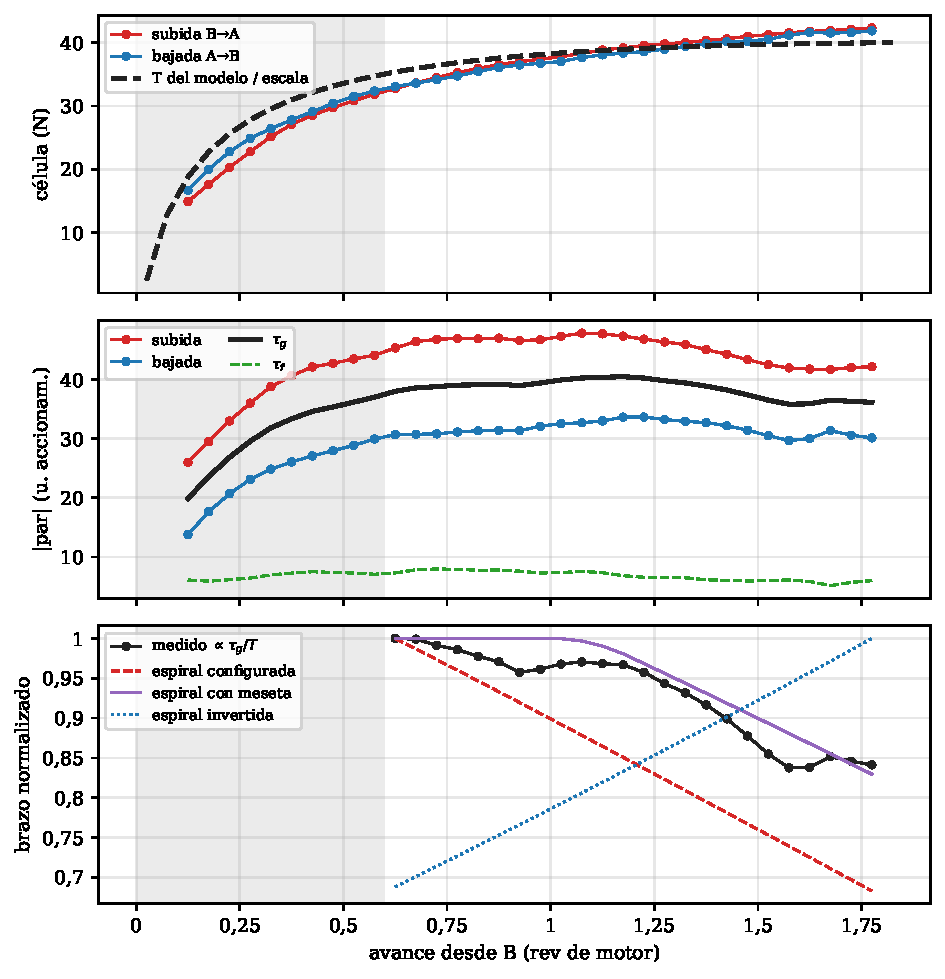
\includegraphics[width=\textwidth]{n14_descomposicion.pdf}
\caption{Promedio de los diez ensayos. Arriba: célula en subida y bajada frente a la tensión del
modelo. Centro: par en los dos sentidos, con el par gravitatorio $\tau_g$ y el de pérdidas $\tau_f$.
Abajo: brazo efectivo deducido de la medida frente a las hipótesis de perfil.}
\label{fig:descomposicion}
\end{figure}

Dos observaciones, ambas sobre el tramo con carga:

\begin{itemize}
  \item \textbf{El par gravitatorio es plano.} Va de \num{38.0} a \num{36.1} unidades de
        accionamiento, es decir \SI{-5}{\percent} a lo largo de todo el tramo, con un valor medio de
        \num{38.5} y un rizado del \SI{12.1}{\percent} en torno a él.
  \item \textbf{Las pérdidas son rozamiento seco.} $\tau_f$ vale \num{6.8} unidades de media y se
        mantiene entre \num{5.2} y \num{8.0} en todo el recorrido, sin tendencia. Es un
        \SI{18}{\percent} del par gravitatorio. Que sea plano, y no proporcional a la velocidad,
        confirma que domina el rozamiento seco y justifica la hipótesis de
        la ecuación~\eqref{eq:separacion}.
\end{itemize}

\subsection{La escala del accionamiento}

Ajustando el par medido al del modelo con una única constante positiva se obtiene
\begin{equation}
  1\ \text{unidad de accionamiento} = \SI{0.0553}{\newton\metre}.
\end{equation}
La cifra merece atención porque es una comprobación cruzada: un ajuste independiente sobre la campaña
de septiembre, con otra geometría y otro tratamiento, daba \SI{0.055}{\newton\metre}. Coinciden
dentro del \SI{1}{\percent}. Con esa escala, el par gravitatorio medio es de
\SI{2.13}{\newton\metre}, el de pico \SI{2.24}{\newton\metre} y el de rozamiento
\SI{0.38}{\newton\metre}. En el eje del motor, con la reducción $N=5$, el pico queda en
\SI{0.45}{\newton\metre}: un \SI{35}{\percent} del par nominal del servomotor. Conviene subrayar que
esta conversión a newton-metro es una cifra \emph{derivada} del ajuste, no una medida independiente;
lo que el accionamiento entrega sin ambigüedad es la forma de la curva y su signo.

\section{Contraste con el modelo: qué perfil explica la medida}
\label{sec:res-contraste}

Éste es el núcleo del trabajo experimental. Se comparan cuatro hipótesis de tambor, todas con la
misma geometría del mecanismo, ajustando en cada caso una única constante positiva de escala:

\begin{enumerate}
  \item \textbf{espiral configurada}, lineal de \num{56} a \SI{28.18}{\milli\metre} en
        \SI{0.367}{rev} de tambor;
  \item \textbf{espiral con meseta}: la misma espiral, precedida de un arco de radio constante
        $r_0$, como la tiene la pieza real;
  \item \textbf{cilindro} de radio constante \SI{44.6}{\milli\metre}, el que recorre lo mismo;
  \item \textbf{espiral invertida}, de \num{28.18} a \SI{56}{\milli\metre}.
\end{enumerate}

\begin{table}[H]
\centering
\caption{Contraste de las hipótesis sobre el tramo con carga. $R^2$ ajusta una sola escala positiva
(ecuación~\eqref{eq:r2-par}); $\rho^2$ es el cuadrado de la correlación, ciego al signo.}
\label{tab:contraste}
\small
\begin{tabularx}{\textwidth}{@{}Xccccc@{}}
\toprule
Hipótesis & \multicolumn{2}{c}{Bondad} & \multicolumn{3}{c}{Predicción sobre el tramo} \\
\cmidrule(lr){2-3}\cmidrule(lr){4-6}
 & $R^2$ & $\rho^2$ & var.\ $\tau$ & var.\ brazo & rizado \\
\midrule
Espiral configurada & \num{-1.23} & \num{0.56} & \SI{-23}{\percent} & \SI{-32}{\percent} & \SI{25.2}{\percent} \\
\textbf{Espiral con meseta} & \textbf{\num{0.84}} & \num{0.85} & \SI{-5}{\percent} & \SI{-17}{\percent} & \SI{13.6}{\percent} \\
Cilindro, \SI{44.6}{\milli\metre} & \num{-1.78} & \num{0.17} & \SI{+15}{\percent} & \SI{0}{\percent} & \SI{13.4}{\percent} \\
Espiral invertida & \num{-20.14} & \num{0.36} & \SI{+72}{\percent} & \SI{+45}{\percent} & \SI{52.4}{\percent} \\
\midrule
\textbf{Medido} & & & \textbf{\SI{-5}{\percent}} & \textbf{\SI{-16}{\percent}} & \textbf{\SI{12.1}{\percent}} \\
\bottomrule
\end{tabularx}
\end{table}

\subsection{La meseta, y por qué la espiral sola no bastaba}

La espiral tal y como está descrita en la configuración predice que el par caiga un
\SI{23}{\percent}; el medido cae un \SI{5}{\percent}. El desacuerdo es grande ($R^2 = \num{-1.23}$,
peor que predecir la media), y sin embargo el sentido es el correcto: el brazo decrece, como dice la
medida. Lo que falla es \emph{cuánto}.

La explicación está en el perfil real. La pieza no empieza a estrecharse en el punto en que arranca
el ensayo: lleva antes un arco de radio constante. Si el cable arranca sobre esa meseta, el tambor
gira un rato sin cambiar de radio y la espiral efectiva es más corta que la nominal. Ajustando la
longitud de esa meseta como único parámetro adicional, el acuerdo salta a $R^2 = \num{0.84}$, y la
meseta que sale vale \SI{0.17}{rev} de tambor, es decir \SI{61}{\degree}. La campaña del 7 de
octubre, analizada igual, da exactamente la misma meseta con $R^2 = \num{0.90}$.

Ese número es el mejor argumento a favor de la hipótesis, porque no se ha usado para construirla:
\emph{el perfil medido sobre el CAD tiene un arco a radio constante de unos \SI{50}{\degree}} antes
de la espiral. El ajuste, que sólo ha visto pares del accionamiento, recupera esa meseta dentro de
una decena de grados.

\subsection{Lo que descarta el cilindro}

El cilindro queda descartado sin ambigüedad ($R^2 = \num{-1.78}$, $\rho^2 = \num{0.17}$). Y lo
descarta por el \emph{sentido}: con radio constante el par sigue a la tensión, que en esta geometría
crece un \SI{15}{\percent}; el par medido no crece, decrece ligeramente. El tambor, por tanto, está
cambiando la relación de transmisión a lo largo del recorrido, que es lo que se quería comprobar.

La espiral invertida es la hipótesis peor con diferencia ($R^2 = \num{-20.1}$): predice que el par
suba un \SI{72}{\percent}. Queda así resuelta en sentido contrario la duda que dejó abierta la
campaña de septiembre, donde el modelo antiguo favorecía precisamente esa orientación.

\subsection{Las dos métricas no dicen lo mismo}

La tabla ilustra de paso por qué la métrica importa. Con $\rho^2$, la espiral configurada puntúa
\num{0.56} y parece una hipótesis aceptable; con $R^2$ y escala positiva es \num{-1.23}. $\rho^2$
premia que la curva tenga la forma adecuada aunque recorra el camino al revés o con la amplitud
equivocada, y aquí eso basta para confundir. Es el mismo aviso que la
sección~\ref{sec:mod-ambiguedad} hace sobre la célula de carga, trasladado al par.

\section{La tensión: célula frente a modelo}

La figura~\ref{fig:modelo}b compara la señal de la célula con la tensión que predice el modelo. El
acuerdo es parcial y conviene ser preciso sobre en qué.

\begin{figure}[tbp]
\centering
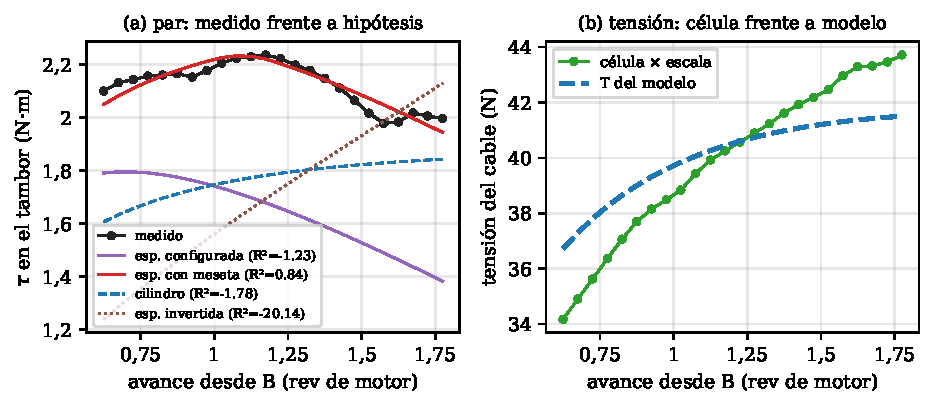
\includegraphics[width=\textwidth]{n14_modelo.pdf}
\caption{(a) Par gravitatorio medido frente a las cuatro hipótesis de tambor. (b) Tensión del cable:
célula de carga, escalada, frente al modelo.}
\label{fig:modelo}
\end{figure}

\textbf{En nivel, coinciden.} Con la calibración provisional del firmware
(\SI{-10.2}{\uacc\per\newton}) la célula da entre \num{33} y \SI{42}{\newton} donde el modelo da
entre \num{37} y \SI{42}{\newton}; el factor de escala que las iguala es \num{1.04}. Para una célula
sin calibrar con masas patrón, un \SI{4}{\percent} es un acuerdo notable, y confirma que el orden
de magnitud del modelo es el correcto.

\textbf{En pendiente, no.} La célula crece un \SI{28}{\percent} a lo largo del tramo con carga, y el
modelo sólo un \SI{13}{\percent}. La discrepancia es sistemática: aparece en los diez ensayos, con
crecimientos medidos entre el \SI{27}{\percent} y el \SI{31}{\percent}, y aparecía igual en la
campaña anterior. No es ruido ni un ensayo aislado.

Lo que sí sostiene la cadena completa es el producto: reconstruyendo el par como fuerza medida por el
brazo del modelo se recupera el par del accionamiento con $R^2 = \num{0.55}$. Es decir, las tres
magnitudes son mutuamente consistentes en primera aproximación, pero queda una discrepancia de
pendiente en la fuerza que el modelo no explica. Las sospechas razonables son la falta de
calibración de la célula ---su sensibilidad podría no ser lineal en este rango--- y el valor de
$e_2$, que es el parámetro al que más responde el brazo del peso. Ninguna de las dos se puede cerrar
sin medir. \verificar{calibrar la célula con masas patrón y medir $\theta_{\text{libre}}$ con
inclinómetro para fijar $e_2$}

\section{Qué aporta realmente el tambor}
\label{sec:res-aporta}

Juntando la medida con la tabla~\ref{tab:perfiles} del capítulo~\ref{chap:modelo} se puede responder
a la pregunta de ingeniería, y la respuesta es más matizada de lo que el planteamiento inicial
suponía.

\begin{itemize}
  \item \textbf{El tambor actúa, y se mide.} El brazo efectivo cae un \SI{16}{\percent} a lo largo
        del tramo con carga, y gracias a eso el par se queda casi plano donde un cilindro lo haría
        subir un \SI{15}{\percent}. El mecanismo hace lo que se diseñó que hiciera.
  \item \textbf{La pieza compensa de más.} Su rizado teórico a igual recorrido es del
        \SI{25}{\percent}, casi el doble que el de un cilindro. Lo que la salva en la práctica es
        precisamente la meseta: el tramo de radio constante acorta la espiral efectiva y deja el
        rizado real en el \SI{12}{\percent} medido.
\end{itemize}

\subsection{Cuánto motor se ahorra, exactamente}
\label{sec:res-ahorro}

La pregunta que importa es cuánto baja el par de pico, por las razones de la
sección~\ref{sec:mod-criterio}. Y admite una respuesta casi sin modelo, apoyada en una identidad:
como el tambor de referencia y el real recorren lo mismo en las mismas vueltas, entregan el mismo
trabajo en el mismo giro y por tanto \emph{tienen el mismo par medio}. Un cilindro, además, copia la
forma de la tensión, porque su radio no cambia. El beneficio se reduce entonces al cociente de dos
relaciones pico/media, ambas medibles:

\begin{table}[H]
\centering
\caption{Relación pico/media sobre el tramo con carga. Como el par medio es el mismo para todos los
tambores que recorren lo mismo en las mismas vueltas, el cociente de estas relaciones es
directamente lo que se ahorra en par de pico.}
\label{tab:picomedia}
\begin{tabular}{@{}lcccc@{}}
\toprule
Magnitud & mín. & media & pico & pico/media \\
\midrule
Par medido (caracola real) & 35,8 & 38,5 & 40,5 & \textbf{1,052} \\
Tensión medida (célula) & 32,9 & 38,5 & 42,1 & 1,094 \\
Tensión del modelo & 36,7 & 40,0 & 41,5 & 1,037 \\
\bottomrule
\end{tabular}
\end{table}

El resultado es modesto y conviene no adornarlo: \textbf{el ahorro en par de pico está entre
\SI{-1.5}{\percent} y \SI{+4}{\percent}}, según se tome la tensión del modelo o la de la célula. Con
el modelo completo, comparando a igual recorrido, el cilindro equivalente (\SI{54.0}{\milli\metre})
pide un \SI{1.5}{\percent} más de pico que la caracola real. En la práctica, en este banco la
caracola no ahorra motor.

La horquilla es, además, otra consecuencia de la discrepancia abierta de la sección anterior: si la
tensión varía el \SI{13}{\percent} que dice el modelo, no hay nada que compensar y la caracola
incluso estorba levemente; si varía el \SI{28}{\percent} que dice la célula, el ahorro es de un
\SI{4}{\percent}. Resolver esa discrepancia es, por tanto, también lo que fijaría el beneficio real.

\subsection{Y el cilindro pequeño, cuantificado}

Queda la objeción natural que plantea la sección~\ref{sec:mod-criterio}: si lo que se busca es menos
par, ¿no bastaría un cilindro más pequeño? La respuesta general es que bajar el radio baja también
el cable por vuelta, y cuesta vueltas. Aquí se puede poner número: el cilindro que iguala el par de
pico de la caracola tiene \SI{53.3}{\milli\metre} y necesita \SI{1.80}{rev} de motor frente a las
\SI{1.77}{rev} de la caracola, es decir, \textbf{un \SI{1}{\percent} más de vueltas}.

Ese \SI{1}{\percent} es la medida exacta de lo que aporta el tambor de radio variable en este banco,
y es despreciable. No porque el principio falle, sino porque \emph{aquí no hay nada que repartir}:
la tensión apenas varía. En un mecanismo donde la tensión variase el doble o el triple ---una barra
que arrancase más abajo, un cable con menos brazo, un muelle en el lazo--- el mismo tambor recortaría
el motor en esa misma proporción. El banco, por tanto, no refuta el principio: lo que demuestra es
que esta geometría concreta no es el caso de uso donde el principio paga.

La conclusión de diseño es que una espiral mucho más suave ---del orden de \num{52} a
\SI{44}{\milli\metre}--- daría a la vez el rizado más bajo (\SI{5.5}{\percent}) y el par de pico más
bajo. Es un cambio barato de aplicar y es la recomendación que se traslada al
capítulo~\ref{chap:conclusiones}.

\section{Limitaciones de las medidas}
\label{sec:res-limitaciones}

\begin{itemize}
  \item La célula no está calibrada con masas patrón. Todo lo que se dice de la fuerza depende de una
        escala ajustada, y por eso el criterio de contraste es el par y no la fuerza.
  \item Las cotas del mecanismo proceden del CAD y de medidas sobre el banco. La más sensible,
        $e_2$, se puede fijar midiendo $\theta_{\text{libre}}$ con un inclinómetro, y conviene
        hacerlo.
  \item La escala del par del accionamiento es un ajuste, no una medida. Un ensayo con un par
        conocido ---una masa colgada de un brazo conocido directamente del eje--- la fijaría.
  \item El modelo es estático y los ensayos se hacen a velocidad constante; el tramo de arranque y
        las inversiones quedan fuera del análisis.
  \item El perfil del tambor se ha tomado de la sección del CAD, no medido sobre la pieza
        fabricada. La meseta ajustada (\SI{61}{\degree}) y la del CAD (\SI{50}{\degree}) difieren en
        una decena de grados, y medir el perfil real cerraría esa diferencia.
\end{itemize}

\section{Trabajo pendiente para cerrar la validación}

Tres medidas, ninguna costosa, convertirían el acuerdo actual en una validación cerrada:

\begin{enumerate}
  \item \textbf{Calibrar la célula} con masas patrón, en el rango de \numrange{0}{60}{} newton. Es
        lo que falta para que la fuerza sea una medida independiente y no una curva escalada.
  \item \textbf{Medir $\theta_{\text{libre}}$} con el cable flojo, y de ahí $e_2$. Es la cota a la
        que más responde el modelo y la que mejor explicaría la discrepancia de pendiente.
  \item \textbf{Levantar el perfil real del tambor}, aunque sea con un calibre y un divisor angular,
        para contrastar la meseta y la ley de la espiral.
\end{enumerate}
